\begin{figure}[ht!]
    \centering
    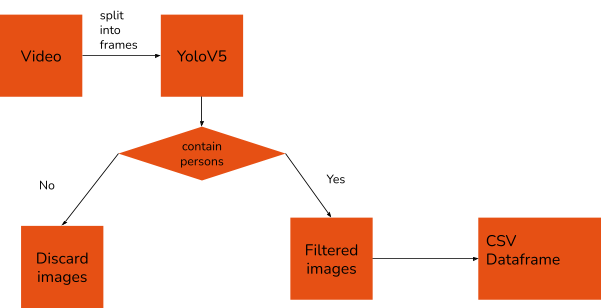
\includegraphics[scale=0.6]{figuras/data_preprocessing.png}
    % \caption[Así aparece el rótulo en el índice]{Así aparece el rótulo en el texto.}
    \caption[Pipeline del procesamiento del conjunto de datos]{Pipeline del procesamiento del conjunto de datos.}
    \label{fig-preprocesamiento-datos}
\end{figure}


Tras la recolección de videos y fotos desde el dispositivo, se realiza un primer proceso de filtrado. Este primer paso consiste en realizar un split de los archivos de video en frames individuales y realizar una operación de reducción del tamaño sobre los frames originales, pasando de 1280 píxeles de ancho y 720 píxeles de alto, a 640 píxeles de ancho y 360 píxeles de alto. Más adelante se tendrá que realizar una segunda reducción de las imágenes para adaptarlas al tamaño de entrada de la red convolucional previa al agente.
\medskip

Este primer paso de filtrado es posible gracias a los algoritmos de detección de objetos, mediante el uso de redes convolucionales neuronales, que nos proporcionan las coordenadas de las bounding box de aquellas clases de objetos que queremos encontrar en nuestro conjunto de datos.
\medskip

Durante el transcurso de nuestro proyecto utilizaremos \textit{YOLOv5}, cuya implementación se encuentra disponible de forma gratuita como librería open source. Dicha implementación nos proporciona además múltiples configuraciones de la red. En nuestro caso, esto no fue muy relevante dado que solo lo utilizaríamos para una primera fase de preprocesamiento de las imágenes.
\medskip

Debido a que la red \textit{YOLOv5} fue entrenada sobre el conjunto de datos \textit{ImageNet} \citep{imagenet} para detectar 1000 clases de objetos diferentes, debemos modificarla para que sea capaz de detectar tan solo una persona en las imágenes que le pasamos, si es que la hay. La documentación de la librería nos ayuda a conseguir esto, de manera que tras una serie de pruebas tanto de diferentes arquitecturas de \textit{YOLO} como de configuración de los parámetros, en concreto: el intervalo de confianza y  el IoU threshold, la red nos devuelve la ubicación de la bounding box en donde se encuentra la persona si es que la hubiese.
\medskip

Sin embargo, para poder adaptar la salida de la red a nuestras necesidades, lo que hicimos fue calcular el punto central de la bounding box en coordenadas X e Y, para que nuestro agente intente acercarse a ese punto durante el entrenamiento en el menor número de pasos posible.
El resultado fue por un lado, un dataframe de Pandas que contenia la ruta de la imagen que \textit{YOLO} había filtrado y las coordenadas X e Y del punto central de la bounding box.
\medskip

Un punto a destacar es que las imágenes que no contenían personas fueron descartadas del conjunto de datos. Esta fue una decisión que se valoró al inicio con el fin de conseguir un agente y una definición más sencilla del problema. De no haber sido así, tendríamos que haber tenido en cuenta el hecho de que la imagen no presenta un punto objetivo y por lo tanto el dron debería permanecer quieto o girar hasta encontrar una persona.
\medskip

El número total de imágenes de nuestro conjunto de datos inicial tras este primer paso se reduce a tan solo 1690 imágenes. Sin embargo, y debido a que nuestro objetivo es modelar los movimientos de giro del dron tenemos que ser conscientes de cuántas imágenes contamos para que el dron nos detecte a la derecha, a la izquierda o en el centro de la imagen.
\medskip

En un primer análisis, nuestro conjunto de datos se encontraba completamente desbalanceado. Lo que hicimos para comprobar esto fue tomar las coordenadas centrales de la bounding box sobre el eje X que calculamos con \textit{YOLO} y comprobar en qué parte de la imagen se encontraba. Si esta coordenada se encontraba entre los píxeles 0 y 280, entonces el dron tendría que que girar a la izquierda, si se encontraba entre el 280 y el 360, entonces podríamos decir que el dron se mantendría prácticamente quieto, y si la coordenada se encontraba por encima de 360, el dron tendría que girar hacia la derecha.
\medskip

Los resultados de este análisis fueron los siguientes:

\begin{itemize}
    \item 340 imágenes se encontraban con la coordenada X en el lado izquierdo.
    \item 870 imágenes se encontraban con la coordenada X en el lado derecho.
    \item 480 imágenes se encontraban con la coordenada X en el centro de la imagen.
\end{itemize}

Debido a este desbalance, se tomó la decisión de igualar la cantidad de imágenes en cada lado, dejando un total de 340 imágenes por cada categoría, lo que hizo un total de 1020 imágenes finales para el entrenamiento y la validación de nuestro agente, lo que en contrapartida podría incrementar aún más el overfitting, pero nos aseguramos de que las decisiones que toma nuestro agente no se verán condicionadas por el número de acciones totales que debería tomar sobre un lado u otro. 
\medskip

Sin embargo, antes de tomar la decisión de descartar las imágenes se estudió la posibilidad también de realizar técnicas de data augmentation tal y como se recomienda en la literatura, utilizando técnicas de crop y volteo horizontal y vertical en cada una de las imágenes, pero la complejidad añadida de tener que recalcular el nuevo punto central hizo que descartemos esa posibilidad.
\medskip

Debido a que nuestro conjunto de datos no es muy grande, decidimos que el conjunto de entrenamiento sea el 90\%, del cual el 80\% se usará para la fase de entrenamiento de nuestro modelo y el otro 20\% se usará para la fase de test. El 10\% restante de nuestro conjunto, aproximadamente 100 imágenes, lo reservamos para la etapa de validación, de manera que probaremos los resultados de nuestro agente sobre un conjunto de imágenes que no haya visto previamente.

